
% This LaTeX was auto-generated from MATLAB code.
% To make changes, update the MATLAB code and republish this document.

\documentclass{article}
\usepackage{graphicx}
\usepackage{color}

\sloppy
\definecolor{lightgray}{gray}{0.5}
\setlength{\parindent}{0pt}

\begin{document}

    
    
\subsection*{Contents}

\begin{itemize}
\setlength{\itemsep}{-1ex}
   \item Sam Nazari
   \item Simulation parameters
   \item Dynamic system
   \item Construct Fault Vectors
   \item UIO 1
   \item UIO 2
   \item Sim \& Plot
\end{itemize}


\subsection*{Sam Nazari}


\begin{verbatim}Teixeira MS Thesis Intrusion Detection Model
06-Nov-2016
04-Jan-2017
12-Jan-2017\end{verbatim}
    \begin{verbatim}
clear,
clc
\end{verbatim}


\subsection*{Simulation parameters}

\begin{verbatim}
TSIM = 20;

% u1Val = 34.632;
% u2Val = 1641.6;
% u3Val = 29980;
%
% X0 = [0.3412;525.7;525.7;496.2];
%
% z110 = 518.6174;
% z410 = -51365.5370;
% z320 = 472.2;
% z420 = -18391.8;
%
% fa1 = 0;
% fa2 = 0;
% fa3 = 1;
%
% f = [fa1;fa2;fa3]
\end{verbatim}


\subsection*{Dynamic system}

\begin{verbatim}
L = [
    3   -1  -1  -1  0   0   0;
    -1  4   -1  -1  -1  0   0;
    -1  -1  3   0   0   -1  0;
    -1  -1  0   3   0   0  -1;
    0   -1  0   0   2   0  -1;
    0   0   -1  0   0   2  -1;
    0   0   0  -1  -1  -1   3
    ]

A = -L

B = eye(7)
Bf=B;
Bf(2,2)=0

C = [
    0 0 0 0 0 0 0;
    0 1 0 0 0 0 0;
    0 0 1 0 0 0 0;
    0 0 0 1 0 0 0;
    0 0 0 0 0 0 0;
    0 0 0 0 0 0 0;
    0 0 0 0 0 0 0
    ]

E = [1.0;20.758;0.0;0.0]

x0 = [0 1 1 0 0 0 0]
\end{verbatim}

        \color{lightgray} \begin{verbatim}
L =

     3    -1    -1    -1     0     0     0
    -1     4    -1    -1    -1     0     0
    -1    -1     3     0     0    -1     0
    -1    -1     0     3     0     0    -1
     0    -1     0     0     2     0    -1
     0     0    -1     0     0     2    -1
     0     0     0    -1    -1    -1     3


A =

    -3     1     1     1     0     0     0
     1    -4     1     1     1     0     0
     1     1    -3     0     0     1     0
     1     1     0    -3     0     0     1
     0     1     0     0    -2     0     1
     0     0     1     0     0    -2     1
     0     0     0     1     1     1    -3


B =

     1     0     0     0     0     0     0
     0     1     0     0     0     0     0
     0     0     1     0     0     0     0
     0     0     0     1     0     0     0
     0     0     0     0     1     0     0
     0     0     0     0     0     1     0
     0     0     0     0     0     0     1


Bf =

     1     0     0     0     0     0     0
     0     0     0     0     0     0     0
     0     0     1     0     0     0     0
     0     0     0     1     0     0     0
     0     0     0     0     1     0     0
     0     0     0     0     0     1     0
     0     0     0     0     0     0     1


C =

     0     0     0     0     0     0     0
     0     1     0     0     0     0     0
     0     0     1     0     0     0     0
     0     0     0     1     0     0     0
     0     0     0     0     0     0     0
     0     0     0     0     0     0     0
     0     0     0     0     0     0     0


E =

    1.0000
   20.7580
         0
         0


x0 =

     0     1     1     0     0     0     0

\end{verbatim} \color{black}
    

\subsection*{Construct Fault Vectors}

\begin{verbatim}
f1 = [1 0 0 0 0 0 0]'  % Vertex one is the intruder
f2 = [0 1 0 0 0 0 0]'  % Vertex two is the intruder
f3 = [0 0 1 0 0 0 0]'  % Vertex three is the intruder
f4 = [0 0 0 1 0 0 0]'  % Vertex four is the intruder
f5 = [0 0 0 0 1 0 0]'  % Vertex five is the intruder
f6 = [0 0 0 0 0 1 0]'  % Vertex six is the intruder
f7 = [0 0 0 0 0 0 1]'  % Vertex seven is the intruder

%E = [f1 f2 f3 f4 f5 f6 f7]
%E = [f2 f3 f4 f5 f6 f7]
E = [f1 f3 f5]

% Choose the agent to be attacked
flt1  = 0
flt2  = 0
flt3  = 0
flt4  = 1
flt5  = 0
flt6  = 0
flt7  = 0

% Choose a magnitude for the attack
f1Val = 10
f2Val = 10
f3Val = 10
f4Val = 10
f5Val = 10
f6Val = 10
f7Val = 10

% Chose the attack time
tf1   = 2
tf2   = 2
tf3   = 2
tf4   = 2
tf5   = 2
tf6   = 5
tf7   = 7
\end{verbatim}

        \color{lightgray} \begin{verbatim}
f1 =

     1
     0
     0
     0
     0
     0
     0


f2 =

     0
     1
     0
     0
     0
     0
     0


f3 =

     0
     0
     1
     0
     0
     0
     0


f4 =

     0
     0
     0
     1
     0
     0
     0


f5 =

     0
     0
     0
     0
     1
     0
     0


f6 =

     0
     0
     0
     0
     0
     1
     0


f7 =

     0
     0
     0
     0
     0
     0
     1


E =

     1     0     0
     0     0     0
     0     1     0
     0     0     0
     0     0     1
     0     0     0
     0     0     0


flt1 =

     0


flt2 =

     0


flt3 =

     0


flt4 =

     1


flt5 =

     0


flt6 =

     0


flt7 =

     0


f1Val =

    10


f2Val =

    10


f3Val =

    10


f4Val =

    10


f5Val =

    10


f6Val =

    10


f7Val =

    10


tf1 =

     2


tf2 =

     2


tf3 =

     2


tf4 =

     2


tf5 =

     2


tf6 =

     5


tf7 =

     7

\end{verbatim} \color{black}
    

\subsection*{UIO 1}

\begin{par}
This UIO is insensitive to faults in agent 2, but can detect faults in agents 3 and 4:
\end{par} \vspace{1em}
\begin{verbatim}
bf1 = [0 1 0 0 0 0 0]'

% Rank conditions
rank(C*bf1)
rank(bf1)

% Observer matrices
CE = C*bf1
CEin = inv(CE'*CE)
H1=bf1*CEin*CE'
T1 = eye(7)-H1*C
A11 = T1*A
rank(obsv(A11,C))
k11 = place(A11,C,[-1,-2,-3,-4,-5,-6,-7])
%F = A1-k1*C
F1 = A+H1*C*L-k11*C
k1 = k11 + F1*H1
\end{verbatim}

        \color{lightgray} \begin{verbatim}
bf1 =

     0
     1
     0
     0
     0
     0
     0


ans =

     1


ans =

     1


CE =

     0
     1
     0
     0
     0
     0
     0


CEin =

     1


H1 =

     0     0     0     0     0     0     0
     0     1     0     0     0     0     0
     0     0     0     0     0     0     0
     0     0     0     0     0     0     0
     0     0     0     0     0     0     0
     0     0     0     0     0     0     0
     0     0     0     0     0     0     0


T1 =

     1     0     0     0     0     0     0
     0     0     0     0     0     0     0
     0     0     1     0     0     0     0
     0     0     0     1     0     0     0
     0     0     0     0     1     0     0
     0     0     0     0     0     1     0
     0     0     0     0     0     0     1


A11 =

    -3     1     1     1     0     0     0
     0     0     0     0     0     0     0
     1     1    -3     0     0     1     0
     1     1     0    -3     0     0     1
     0     1     0     0    -2     0     1
     0     0     1     0     0    -2     1
     0     0     0     1     1     1    -3


ans =

     7


k11 =

         0         0         0         0         0         0         0
    0.4469    7.0316   -0.0797    0.4125    0.3204    0.0027    0.1221
    0.8230    0.5890    2.4289   -0.7112   -0.0196    0.8962   -0.1124
    0.9040    1.1596   -0.6336    2.5395    0.1004   -0.0957    0.9599
         0         0         0         0         0         0         0
         0         0         0         0         0         0         0
         0         0         0         0         0         0         0


F1 =

   -3.0000    1.0000    1.0000    1.0000         0         0         0
         0   -7.0316    0.0797   -0.4125         0         0         0
    1.0000    0.4110   -5.4289    0.7112         0    1.0000         0
    1.0000   -0.1596    0.6336   -5.5395         0         0    1.0000
         0    1.0000         0         0   -2.0000         0    1.0000
         0         0    1.0000         0         0   -2.0000    1.0000
         0         0         0    1.0000    1.0000    1.0000   -3.0000


k1 =

         0    1.0000         0         0         0         0         0
    0.4469         0   -0.0797    0.4125    0.3204    0.0027    0.1221
    0.8230    1.0000    2.4289   -0.7112   -0.0196    0.8962   -0.1124
    0.9040    1.0000   -0.6336    2.5395    0.1004   -0.0957    0.9599
         0    1.0000         0         0         0         0         0
         0         0         0         0         0         0         0
         0         0         0         0         0         0         0

\end{verbatim} \color{black}
    

\subsection*{UIO 2}

\begin{par}
This UIO is insensitive to faults in agent 3, but can detect faults in agents 2 and 4:
\end{par} \vspace{1em}
\begin{verbatim}
bf2 = [0 0 1 0 0 0 0]'

% Rank conditions
rank(C*bf2)
rank(bf2)

% Observer matrices
CE = C*bf2
CEin = inv(CE'*CE)
H2=bf2*CEin*CE'
T2 = eye(7)-H2*C
A12 = T2*A
rank(obsv(A12,C))
k12 = place(A12,C,[-1,-2,-3,-4,-5,-6,-7])
%F = A1-k1*C
F2 = A+H2*C*L-k12*C
k2 = k12 + F2*H2
\end{verbatim}

        \color{lightgray} \begin{verbatim}
bf2 =

     0
     0
     1
     0
     0
     0
     0


ans =

     1


ans =

     1


CE =

     0
     0
     1
     0
     0
     0
     0


CEin =

     1


H2 =

     0     0     0     0     0     0     0
     0     0     0     0     0     0     0
     0     0     1     0     0     0     0
     0     0     0     0     0     0     0
     0     0     0     0     0     0     0
     0     0     0     0     0     0     0
     0     0     0     0     0     0     0


T2 =

     1     0     0     0     0     0     0
     0     1     0     0     0     0     0
     0     0     0     0     0     0     0
     0     0     0     1     0     0     0
     0     0     0     0     1     0     0
     0     0     0     0     0     1     0
     0     0     0     0     0     0     1


A12 =

    -3     1     1     1     0     0     0
     1    -4     1     1     1     0     0
     0     0     0     0     0     0     0
     1     1     0    -3     0     0     1
     0     1     0     0    -2     0     1
     0     0     1     0     0    -2     1
     0     0     0     1     1     1    -3


ans =

     7


k12 =

         0         0         0         0         0         0         0
    1.4469    3.0316    0.9203    1.4125    1.3204    0.0027    0.1221
   -0.1770   -0.4110    5.4289   -0.7112   -0.0196   -0.1038   -0.1124
    0.9040    1.1596   -0.6336    2.5395    0.1004   -0.0957    0.9599
         0         0         0         0         0         0         0
         0         0         0         0         0         0         0
         0         0         0         0         0         0         0


F2 =

   -3.0000    1.0000    1.0000    1.0000         0         0         0
    1.0000   -7.0316    0.0797   -0.4125    1.0000         0         0
         0    0.4110   -5.4289    0.7112         0         0         0
    1.0000   -0.1596    0.6336   -5.5395         0         0    1.0000
         0    1.0000         0         0   -2.0000         0    1.0000
         0         0    1.0000         0         0   -2.0000    1.0000
         0         0         0    1.0000    1.0000    1.0000   -3.0000


k2 =

         0         0    1.0000         0         0         0         0
    1.4469    3.0316    1.0000    1.4125    1.3204    0.0027    0.1221
   -0.1770   -0.4110         0   -0.7112   -0.0196   -0.1038   -0.1124
    0.9040    1.1596         0    2.5395    0.1004   -0.0957    0.9599
         0         0         0         0         0         0         0
         0         0    1.0000         0         0         0         0
         0         0         0         0         0         0         0

\end{verbatim} \color{black}
    

\subsection*{Sim \& Plot}

\begin{verbatim}
sim('TeixeiraModel')

figure,
subplot(311),
plot(fn2),ylabel('r12'),xlabel('Time (sec)'),title('Residual Signal for Node 2'), grid on, ylim([-5,5])
subplot(312),
plot(fn3),ylabel('r13'),xlabel('Time (sec)'),title('Residual Signal for Node 3'), grid on, ylim([-5,5])
subplot(313),
plot(fn4),ylabel('r14'),xlabel('Time (sec)'),title('Residual Signal for Node 4'), grid on, ylim([-5,5])
%
% figure,
% subplot(311),
% plot(tout,y1R,'k'),ylabel('y1_R'),xlabel('Time (sec)'),title('Outputs: y1_R, y2_R, y3_R')
% subplot(312),
% plot(tout,y2R,'b'),ylabel('y2_R'),xlabel('Time (sec)')
% subplot(313),
% plot(tout,y3R,'r'),ylabel('y3_R'),xlabel('Time (sec)')
%
% figure,
% plot(tout,r11,'k'),ylabel('r_1^1'),xlabel('Time (sec)')
% title('Residual from UIO 1')
%
% figure,
% plot(tout,r12,'k'),ylabel('r_1^2'),xlabel('Time (sec)')
% title('Residual from UIO 2')
%
% figure
% ax1=subplot(411),plot(tout,y1R*T1(1,1),'k'),ylabel('y1R x T_1(1,1)')
% grid on
% ax2=subplot(412),plot(tout,y2R,'r'),ylabel('y2R')
% grid on
% ax3=subplot(413),plot(tout,z11,'b'),ylabel('z_1^1'),
% grid on
% ax4=subplot(414),plot(tout,r11,'g'),ylabel('r_1^1'),
% grid on
% linkaxes([ax1,ax2,ax3,ax4],'x')
%
% figure,
% ax1=subplot(211),plot(tout,r11,'k'),ylabel('r_1^1'),
% title('Residual from UIO 1 and UIO 2'),xlabel('Time (hr)')
% grid on
% ax2=subplot(212),plot(tout,r12,'b'),ylabel('r_1^2')
% xlabel('Time (hr)'),grid on
% linkaxes([ax1,ax2],'x')
% figure
% ax1=subplot(411),plot(tout,y1R*T1(1,1),'k'),ylabel('y1R x T_1(1,1)')
% grid on
% ax2=subplot(412),plot(tout,y2R,'r'),ylabel('y2R')
% grid on
% ax3=subplot(413),plot(tout,z11,'b'),ylabel('z_1^1'),
% grid on
% ax4=subplot(414),plot(tout,r11,'g'),ylabel('r_1^1'),
% grid on
% linkaxes([ax1,ax2,ax3,ax4],'x')

%
% figure,
% plot(tout,r2)
\end{verbatim}

        \color{lightgray} \begin{verbatim}Warning: Model 'TeixeiraModel' is using a default value of 0.2 for maximum step
size. You can disable this diagnostic by setting 'Automatic solver parameter
selection' diagnostic to 'none' in the Diagnostics page of the configuration
parameters dialog 
\end{verbatim} \color{black}
    
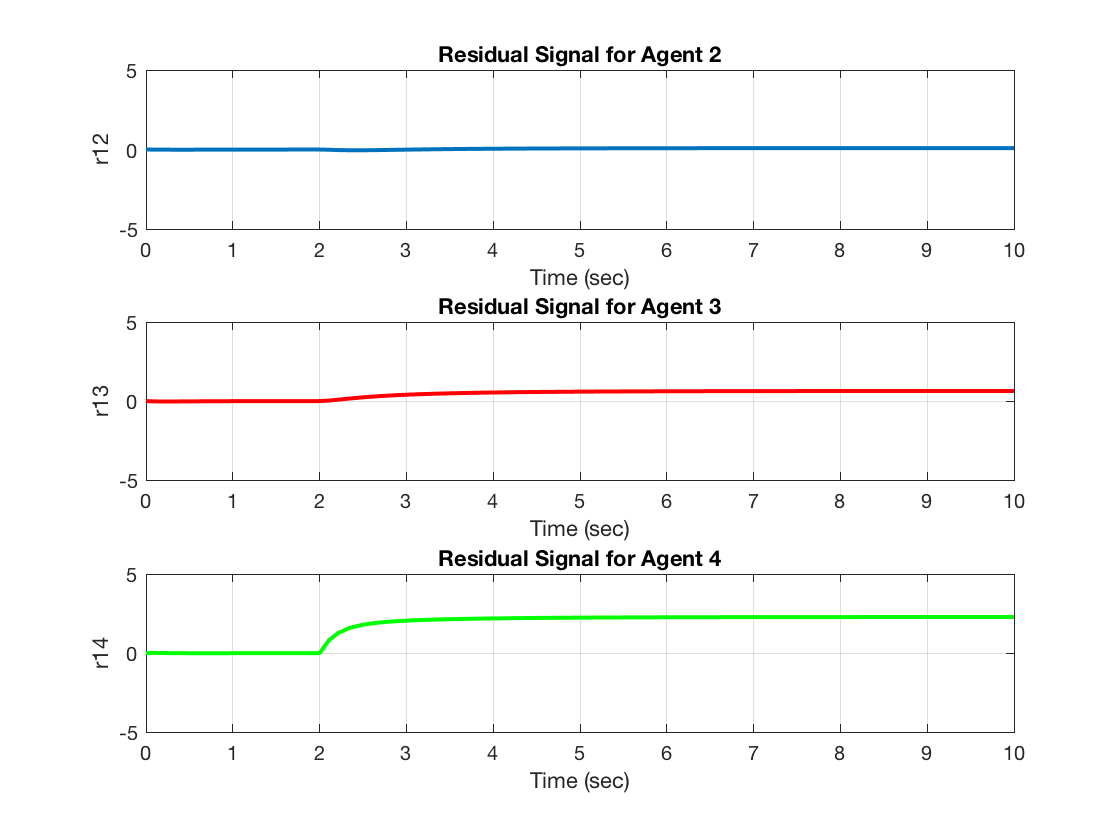
\includegraphics [width=4in]{intrusionDetectionMS_01.eps}



\end{document}
    
